\documentclass{beamer}
\usepackage[utf8]{inputenc}
% \usepackage[english]{babel}
\usepackage{hyperref}
\usepackage{graphicx}
\graphicspath{{../../../output/figures/Presentation/}}
\usepackage{wrapfig}
\usepackage{subcaption}
\usepackage{booktabs}
\usepackage[space]{grffile}
\usepackage{amsmath,amssymb,bbm}
\def\Min{\mathop{\rm Min}}
\def\Max{\mathop{\rm Max}}
\def\bbe{{\Bbb{E}}}
\def\bbe{{\Bbb{E}}}
% \usepackage[square,numbers]{natbib}
%\bibliographystyle{unsrtnat}
\usepackage{pifont}
\usepackage{xcolor}
\newcommand{\cmark}{\textcolor{green!80!black}{\ding{51}}}
\newcommand{\xmark}{\textcolor{red}{\ding{55}}}

\makeatletter
\let\@@magyar@captionfix\relax
\makeatother
\newtheorem{defn}[theorem]{Definition}
\DeclareMathOperator*{\argmax}{arg\,max}
\DeclareMathOperator*{\argmin}{arg\,min}
\hypersetup{
    allcolors={}
}

\usetheme{Boadilla}
\usecolortheme{beaver}

\usepackage[
backend=biber,
style=bwl-FU,
sorting=ynt
]{biblatex}
\addbibresource{../../main.bib}

\title[Agricultural Index Insurance]{Agricultural Index Insurance: An Optimization Approach}
\author[José Velarde Morales]{José I. Velarde Morales}
\institute[Chicago Booth]
{

  University of Chicago\\
  Booth School of Business

}


\begin{document}
\beamertemplatenavigationsymbolsempty
\frame{\titlepage}
\section{Introduction}
\subsection*{The Problem of Agricultural Risk}
\begin{frame}{The Problem of Agricultural Risk}
\begin{itemize}
    \setlength\itemsep{2em}
    \item Farmers face a lot of risk, and the lack of risk management tools forces them to use coping strategies that hurt their long term welfare.
   
    \item Traditional insurance is prohibitively costly in most developing countries due to lack of data and high verification costs.

    \item Moral hazard, adverse selection, and the presence of large covariate shocks make the problem of agricultural insurance especially hard. 
\end{itemize}
\end{frame}

\subsection*{A Proposed Solution: Index Insurance}
\begin{frame}{A Proposed Solution: Index Insurance}
\begin{itemize}
   \setlength\itemsep{1em}
    % \item Researchers developed index insurance as a less costly way to offer insurance in developing countries. 
    \item In index insurance, an index (or statistic) is created using easily observable quantities (e.g. rainfall), and it is used to determine whether the insured party suffered an adverse event. 
    \item If the index falls below a pre-determined threshold, the insurer automatically issues out payments to the insured. 
    \item This allows the insurer to circumvent the issue of verification and moral hazard, since the actions of individual farmers cannot affect the index.
\end{itemize}
\end{frame}

\begin{frame}{Index Insurance in Practice}
    \begin{itemize}
        \setlength\itemsep{1.5em}
        \item Since it was first proposed, index insurance programs have been implemented in many countries including India, Mexico, Tanzania, Malawi, Kenya, and many others (\cite{jensen2017agricultural}). 
        
        \item Today, tens of millions of farmers worldwide are covered by index insurance programs (\cite{greatrex2015scaling}). 
        
        \item However, in most of these cases, the insurance has to be heavily subsidized by governments due to high cost and low demand (\cite{greatrex2015scaling}). 
    \end{itemize}
    \end{frame}

    

% \subsection*{Project Overview}
% \begin{frame}{Project Overview}
%  \begin{itemize}
%     \setlength\itemsep{1em}   
%     % \item Traditionally, contracts are designed to maximize correlation between payouts and losses (\cite{chantarat2013designing}).  %This ignores valuable information about the correlation between zones that affects the cost of insuring the whole portfolio. 
%     \item The goal of this project is to improve the design of index insurance contracts. I am particularly interested in the developing country setting.  
%     \item The original motivation was to develop a method to simultaneously design contracts for all insured zones, in order to better manage risk. However, upon learning more about the context I realized that the optimization based approach could be an improvement even in the single zone case. 
%     \item We develop a method that tries to maximize farmer utility, incorporates different kinds of constraints, and yields interpretable contracts. 
%     % \item Our method simultaneously determines the contract parameters for different areas, while taking into account the correlation between the areas, reducing risk for the insurer. 
%  \end{itemize}
% \end{frame}

% \begin{frame}{Motivation for multi-zone optimization}
%     \begin{itemize}
%         \item For the insurer, the risk (and therefor cost) of providing a line of insurance depends on the other lines of insurance in its portfolio. 
%         \item If all of its lines of insurance are highly correlated, it will be more expensive due to capital requirements. 
%         \item This is similar to the problem of portfolio design, where the correlations between stocks affect optimal portfolio composition. 
%         \item Insurers can influence the composition of their portfolio through the contracts they offer, so they should be better able to manage
%         their costs if they take into account the correlation of different lines of insurance when designing contracts.
%     \end{itemize}
    
% \end{frame}

\section{Background}
\begin{frame}[noframenumbering, plain]
    \frametitle{Content}
    \tableofcontents[currentsection]
  \end{frame}
\subsection{Index Insurance Background}
\begin{frame}{Index Insurance: General Context}
    \begin{itemize}
        \setlength\itemsep{1em}
        \item Index insurance is a named-peril insurance.
        \item It is often tied to access to credit.
        \item Offered at different levels (micro level, meso level, and macro level)
        \item Often based on public-private partnerships. Research institutions usually design the product, and insurance companies (or governments) sell it. 
    \end{itemize}
    \end{frame} 

\begin{frame}{Index Insurance: Definition and Parameters}
    \begin{itemize}
        \setlength\itemsep{1em}
        \item Index insurance uses a signal, $\theta$, to predict agricultural loss, $\hat{\ell}(\theta)$
        \item Contract form: $I(\hat{\ell}(\theta)) = \min \left \{ \max \left \{a\hat{\ell}(\theta) - b,0 \right \}, 1 \right \}$, $a,b$ are the contract parameters.
        % \item Expected cost for insurer: $C(I(\theta)) = \mathbb{E}[I(\theta)] + c_{\kappa} K(I(\theta))$, where $c_{\kappa}$ is the cost of capital, and $K$ is required capital.
        % \item $K(I(\theta)) = CVaR_{1-\epsilon_P}\left ( I(\theta) \right ) - \mathbb{E}[I(\theta)]$.
    \end{itemize}
    \end{frame}

    \begin{frame}{Reasoning for piecewise linear contracts}
        \begin{itemize}
            \setlength \itemsep{2em}
            \item Research has consistently found that contract copmrehension is key for take up (\cite{cole2013barriers}; \cite{ahmed2020impact}) 
            \item Deductible insurance is theoretically optimal (\cite{arrow1974optimal})
            \item Widely used in practice (\cite{gamage2021index}; \cite{world2011weather})
        \end{itemize}
    \end{frame}
    
    \begin{frame}{Example of Index Insurance Contract}
        \begin{figure}
            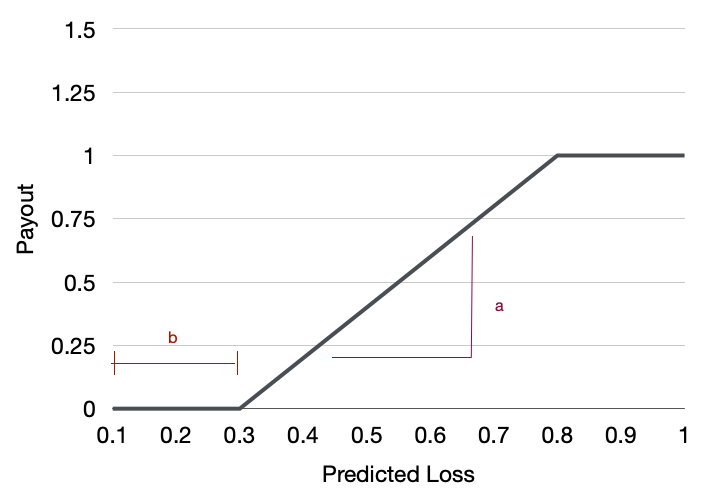
\includegraphics[width=0.9\textwidth]{../../../output/figures/Presentation/sample_insurance_contract.png}
        \end{figure}
    \end{frame}

    \begin{frame}{Motivation for multi-zone optimization}
        Insurer's expected costs for insuring its entire portfolio are:
        \begin{align*}
            C = \mathbb{E}\left [ \sum_z s_z I_z (\hat{\ell_z}) \right ] + c_{\kappa} R \left (\sum_z s_z I_z(\hat{\ell_z}) \right )
        \end{align*}

        Charges per-unit premium of:
        \begin{align*}
            \pi_z = \mathbb{E}\left [ \sum_z I_z (\hat{\ell_z}) \right ] +  c_{\kappa} \frac{\beta_z}{s_z} R \left (\sum_z s_z I_z(\hat{\ell_z}) \right )
        \end{align*}

        Where $R(\cdot)$ is a risk measure capturing capital requirements, $s_z$ is the number of insured units in zone $z$, and $\beta_z$ is the share of the capital costs paid by zone $z$. 
    \end{frame}

    \begin{frame}{Insurer's Optimization Problem}

        Insurer wants to find $\mathbf{a} = (a_1,...,a_
        Z), \mathbf{b}= (b_1, ...,b_Z)$ that will maximize overall utility.
        \begin{align*}
            \max_{\mathbf{a},\mathbf{b}}  & \quad \mathbb{E} \left [ \sum_z s_z u\left ( w_0 + 1 - \ell_z - \pi_z + I_z(\hat{\ell_z}) \right ) \right ] \\
    \text{s.t.} & \quad \pi_z = \mathbb{E}\left [ I_z (\hat{\ell_z}) \right ] +  c_{\kappa} \frac{\beta_z}{s_z} R \left (\sum_z s_z I_z(\hat{\ell_z}) \right )\\
        \end{align*}

        FOC's for $a_z$:
        \begin{align*}
            \frac{\partial I_z}{\partial a_z} - \mathbb{E} \left [ \frac{\partial I_z}{\partial a_z} \right ] = c_{\kappa} \beta_z R' \left (\sum_z s_z I_z(\hat{\ell_z}) \right ) \frac{\partial I_z}{\partial a_z}
        \end{align*}
        
    \end{frame}

    \begin{frame}{Insurer's Optimization in Single Zone Case}
        If designing the contracts independently, the insurer's optimization problem becomes:
        \begin{align*}
            \max_{a,b}  & \quad \mathbb{E} \left [ u\left ( w_0 + 1 - \ell_z - \pi_z + I_z(\hat{\ell_z}) \right ) \right ] \\
    \text{s.t.} & \quad \pi_z = \mathbb{E}\left [ I_z (\hat{\ell_z}) \right ] +  c_{\kappa} \frac{\beta_z}{s_z} R \left ( s_z I_z(\hat{\ell_z}) \right )\\
        \end{align*}
        
    FOC's for $a_z$:
        \begin{align*}
            \frac{\partial I_z}{\partial a_z} - \mathbb{E} \left [ \frac{\partial I_z}{\partial a_z} \right ] = c_{\kappa} R' \left (s_z I_z(\hat{\ell_z}) \right ) \frac{\partial I_z}{\partial a_z}
        \end{align*}

    \end{frame}

    \begin{frame}{Comparing FOC's}
        Multi-zone Optimization FOC's:
        \begin{align*}
            \frac{\partial I_z}{\partial a_z} - \mathbb{E} \left [ \frac{\partial I_z}{\partial a_z} \right ] = c_{\kappa} \beta_z R' \left (\sum_z s_z I_z(\hat{\ell_z}) \right ) \frac{\partial I_z}{\partial a_z}
        \end{align*}

        Single-zone Optimization FOC's:
        \begin{align*}
            \frac{\partial I_z}{\partial a_z} - \mathbb{E} \left [ \frac{\partial I_z}{\partial a_z} \right ] = c_{\kappa} R' \left (s_z I_z(\hat{\ell_z}) \right ) \frac{\partial I_z}{\partial a_z}
        \end{align*}
        
    \end{frame}

    \begin{frame}{FOC's when $R(\cdot) = sd(\cdot)$ and $|Z|=2$}
        Multi-zone Optimization FOC's:
        \begin{align*}
            \hat{\ell_1} - \mathbb{E} \left [ \hat{\ell_1} \right ] = c_{\kappa} \beta_1 \hat{\ell_1} \frac{\left ( a_1 Var(\hat{\ell_1}) + a_2 Cov(\hat{\ell_1},\hat{\ell_2}) \right )}{\sqrt{a_1^2 Var(\hat{\ell_1}) + a_2^2 Var(\hat{\ell_2}) +2a_1a_2 Cov(\hat{\ell_1},\hat{\ell_2}) }}
        \end{align*}

        Single-zone Optimization FOC's:
        \begin{align*}
            \hat{\ell_1} - \mathbb{E} \left [ \hat{\ell_1} \right ] = c_{\kappa} \hat{\ell_1} sd(\hat{\ell_1})
        \end{align*}
    \end{frame}

\subsection{Literature Review}
\begin{frame}{Index Insurance Literature}
    \begin{itemize}
        \item \textbf{Impact of Index Insurance:} Overall, there is evidence that index insurance reduces reliance on detrimental risk-coping strategies, increases investment, and leads to riskier, but more profitable production decisions (\cite{jensen2017agricultural};  \cite{cole2013barriers}; \cite{mobarak2013informal}; \cite{karlan2014agricultural}).
        \item \textbf{Demand for Index Insurance:} Demand for index insurance tends to be low and highly price sensitive (\cite{jensen2017agricultural};  \cite{cole2013barriers}; \cite{cai2020subsidy},\cite{casaburi2018time}).
        \item \textbf{Design of Index Insurance:} There has been relatively little research studying the design of index insurance. The method developed by \cite{chantarat2013designing} is the most commonly used in academic publications (\cite{jensen2019does};  \cite{flatnes2018improving}). More recently, \cite{chen2023managing} used a NN approach for contract design. 
    \end{itemize}
   \end{frame}


\subsection{Current Approaches}
\begin{frame}{Baseline Method: \cite{chantarat2013designing}}
    Developed by \cite{chantarat2013designing}, used in Kenya Index Based Livestock Insurance (IBLI) program.  Consist of two steps: 
    \vspace{5mm}
    \begin{enumerate}
        \item Train model to predict loss
        \item Choose strike value, $b$, that maximizes correlation between payouts and losses
    \end{enumerate}

    \vspace{5mm}
    \textbf{Pros:} simple, interpretable \\
    \textbf{Cons:} can't incorporate constraints, doesn't take into account premium 
    
\end{frame}

\begin{frame}{Baseline Method Flowchart}
    \begin{figure}
        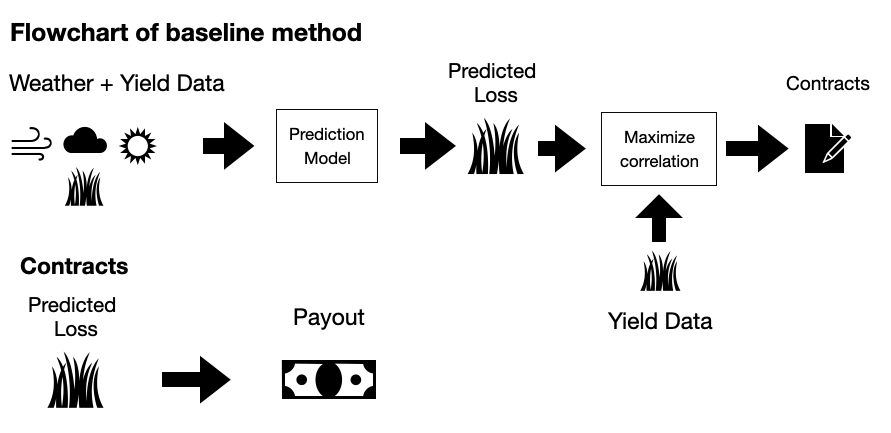
\includegraphics[width=\textwidth]{../../../output/figures/Baseline Flowchart 2.png}
    \end{figure}
    
\end{frame}

\begin{frame}{NN Approach: \cite{chen2023managing}}
    Train neural network to solve the following optimization problem: 
    \begin{align*}
        \max &\quad \mathbb{E} \left [ u(w_0 + 1 - \ell + I -\pi) \right ]\\
        \text{s.t.} & \quad \pi = \lambda \mathbb{E}\left [ I \right ]\\
        & \quad \pi \leq \overline{\pi}
    \end{align*}

    Use CARA utility function:
    \begin{align*}
        & u(w) = \frac{-1}{\alpha} e^{-\alpha w}\\
        & \alpha > 0
    \end{align*}
\end{frame}

\begin{frame}{NN Approach: Cont'd}
    \begin{itemize}
        \setlength\itemsep{2em}
        \item Use a feed forward NN with 3 hidden layers of size 64-64-16.
        \item Evaluate their method using corn yield data from the US Midwest. 
        \item \textbf{Pros:} Directly maximizes utility, admits price constraints. 
        \item \textbf{Cons:} Not interpretable. hard to adjust, large data requirements 
    \end{itemize}
    
\end{frame}

\begin{frame}{NN Approach Flowchart}
    \begin{figure}
        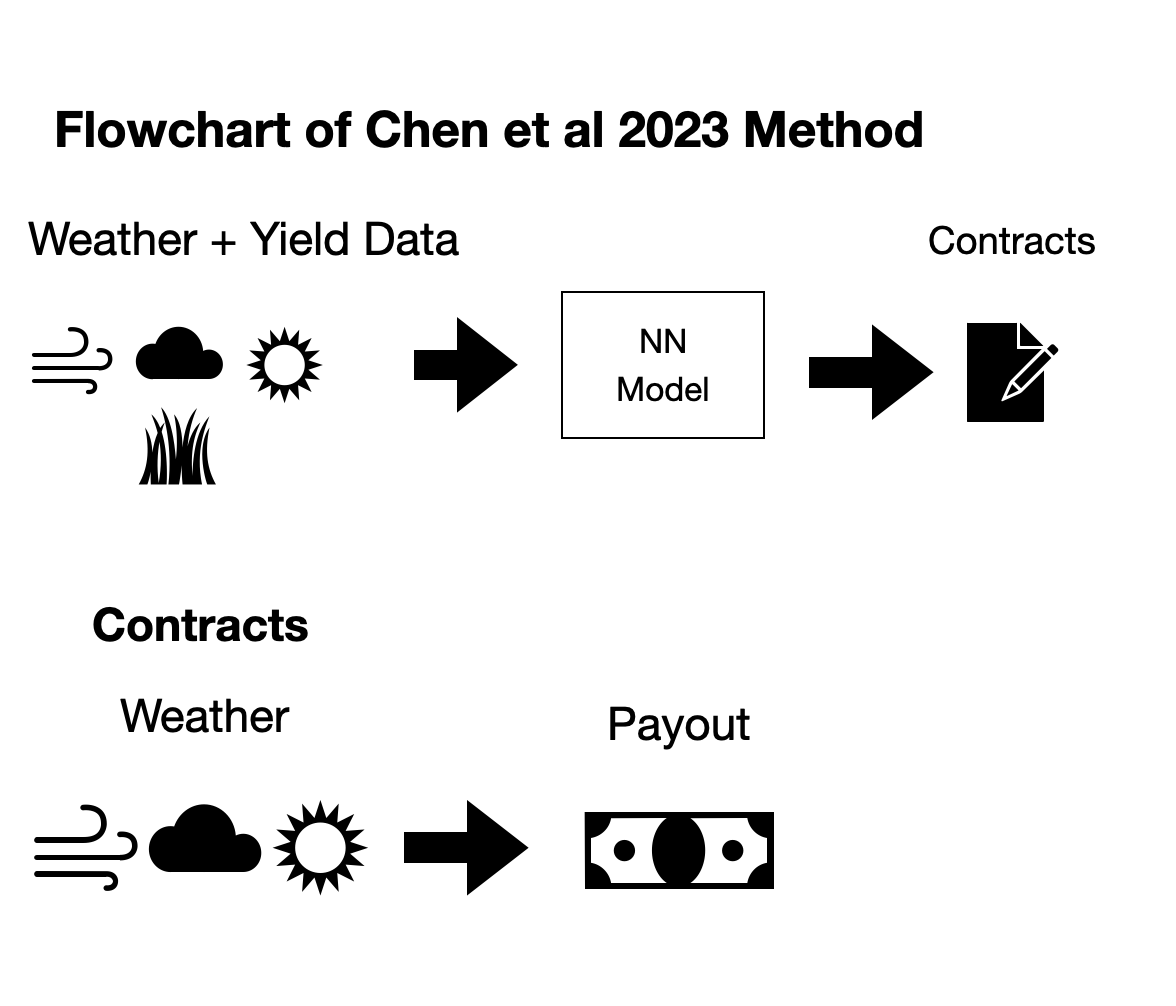
\includegraphics[width=0.8\textwidth]{../../../output/figures/Chen Flowchart.png}
    \end{figure}
    
\end{frame}



% \begin{frame}{Current methods to design index insurance}
% \begin{itemize}
%     \setlength\itemsep{1em}
%     \item \textbf{Baseline Method:} Predict then design, design contracts to maximize correlation between payouts and losses. \cite{chantarat2013designing}
%     \begin{itemize}
%         \item \textbf{Pros:} simple, interpretable
%         \item \textbf{Cons:} can't incorporate constraints
%     \end{itemize}
%     \item \textbf{NN Based Method:} End to end, use NN to design contracts. Combine prediction and contract design into single step. \cite{chen2023managing}
%     \begin{itemize}
%         \item \textbf{Pros:} directly maximizes utility, admits price contstraints
%         \item \textbf{Cons:} not interpretable, hard to adjust, requires a lot of data to train. 
%     \end{itemize}
% \end{itemize}
% \end{frame} 

% \begin{frame}{Drawbacks of current methods}
%     \begin{itemize}
%         \setlength\itemsep{1em}
%         \item \textbf{Baseline Method:} 
%         \begin{itemize}
%             \item Can't incorporate constraints
%             \item Only adjusts one contract parameter
%         \end{itemize}
%         \item \textbf{NN Based Method:} 
%         \begin{itemize}
%             \item Not interpretable, can't set constraints on variables that policy makers might care about (e.g. deductible). This also makes it hard to debug: is the performance due to poor prediction performance? Too high a deductible? 
%             \item Requires a lot of data to train (model has 10,000 parameters)
%             \item Premium definition used only considers expected value of payouts. In practice, variance is highly important. 
%         \end{itemize}
%     \end{itemize}
%     \end{frame} 

\section{Optimization Approach}
\begin{frame}[noframenumbering, plain]
    \frametitle{Content}
    \tableofcontents[currentsection]
  \end{frame}

  \begin{frame}{Our Approach: Overview}
    Our approach is most similar to the baseline method. We predict-then-design. The steps are: 
    \vspace{5mm}
    
    \begin{enumerate}
        \item Train a traditional ML model to predict loss
        \item Use model predictions and ground truth to design contracts
    \end{enumerate}
    
    \vspace{5mm}
    This yields simple and interpretable contracts. 
  \end{frame}

  \begin{frame}{Overview}
    \begin{itemize}
        \setlength\itemsep{2em}
        \item We opt for a "predict-then-optimize" approach.
        \item We use specialized time-series feature extraction algorithms and traditional ML algorithms (e.g. Random Forest, Gradient Boosting, Support Vector Machines) to build a loss prediction model.
        \item We then use model predictions and actual losses to design contracts to maximize utility. 
    \end{itemize}
\end{frame}

% \begin{frame}{Benefits of Our Approach}
%     \begin{itemize}
%         \setlength\itemsep{2em}
%         \item Admits price constraints and payout frequency constraints
%         \item Yields simple, adjustable, and interpretable contracts
%         \item Flexibility: it can use different prediction models and premium definitions
%         \item Requires less data to train than NN approach. 
%     \end{itemize}
% \end{frame}

\begin{frame}{Method Comparison}
    \begin{table}
        \centering
    \begin{tabular}{c|c|c|c|}  
        \multicolumn{1}{c|}{} & Baseline & Chen & VMX  \\
        \hline
        Simple contracts & \cmark & \xmark & \cmark \\
        \hline
        Adjustable contracts & \cmark & \xmark & \cmark \\
        \hline
        Price constraints & \xmark & \cmark & \cmark \\
        \hline
        Payout frequency constraints & \xmark & \xmark & \cmark \\
        \hline
        Different premiums defn's & \xmark & \cmark & \cmark \\
        \hline
        Multi-zone contract design & \xmark & \xmark & \cmark \\
        \hline
    \end{tabular}
\end{table}
\end{frame}

\begin{frame}{Our Method Flowchart}
    \begin{figure}
        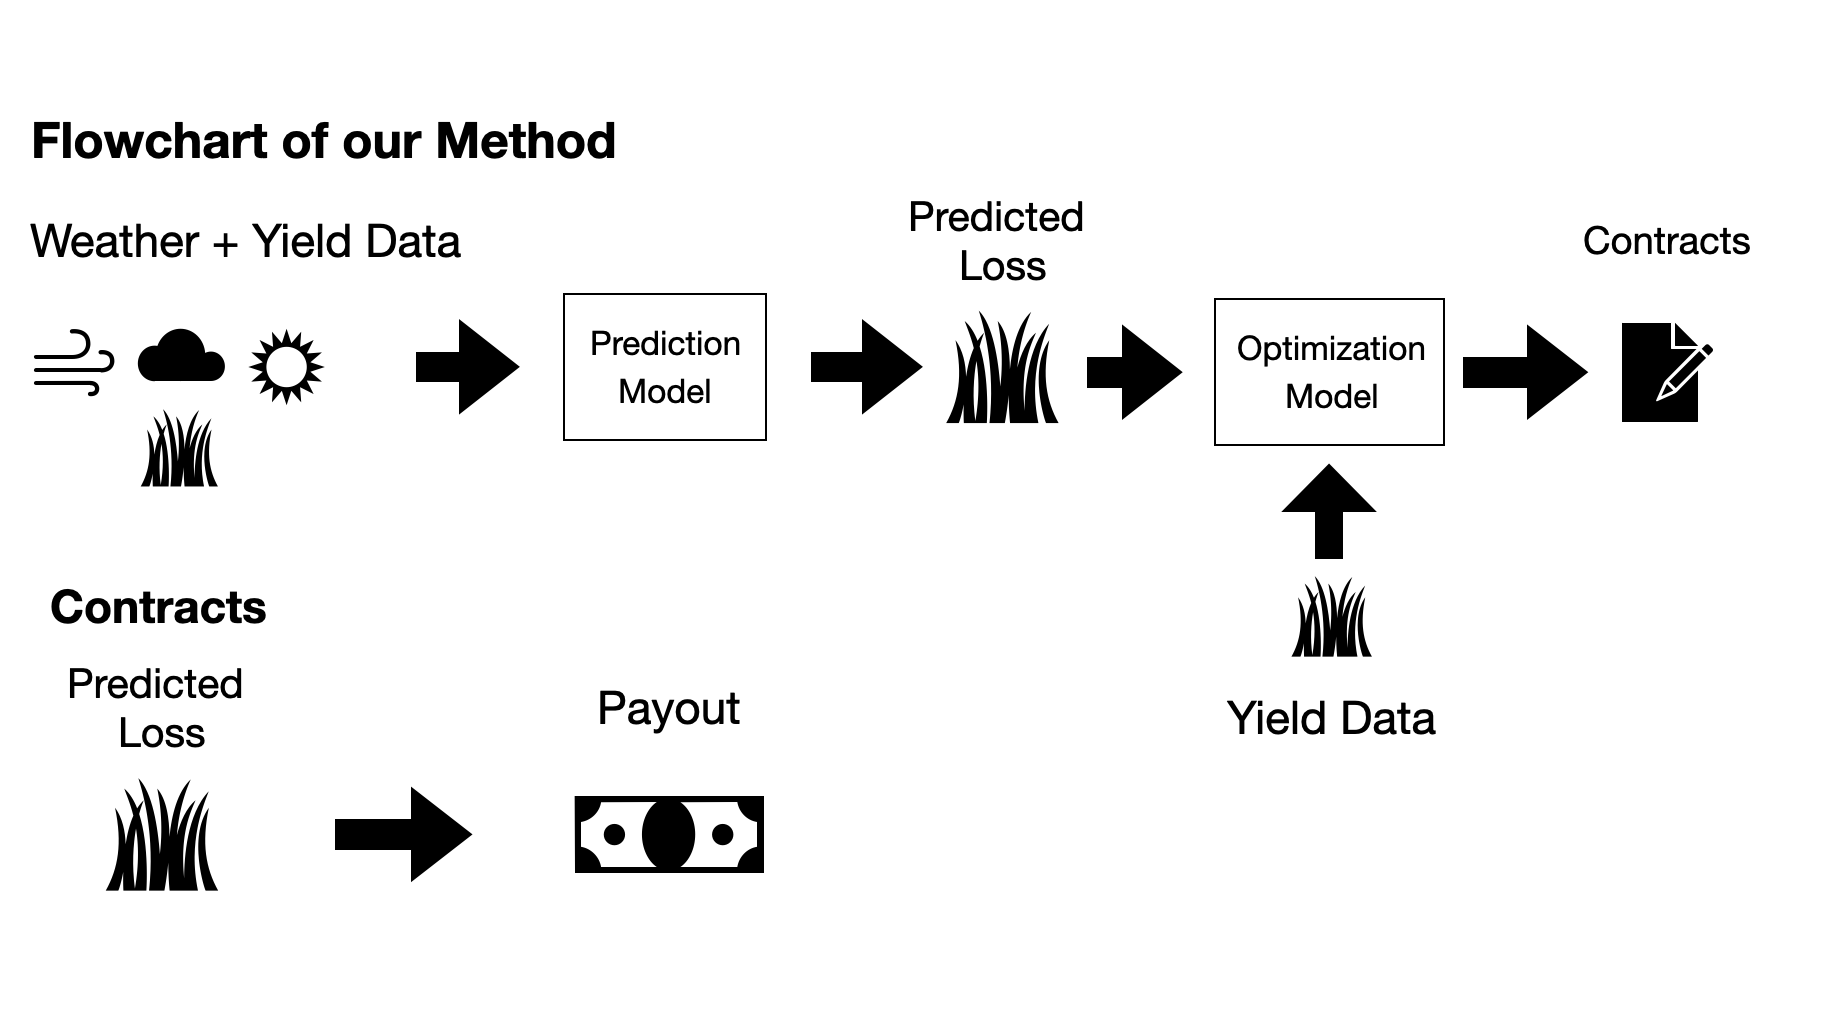
\includegraphics[width=\textwidth]{../../../output/figures/Our Method Flowchart.png}
    \end{figure}
\end{frame}

% \begin{frame}{Benefits of Our Approach}
%     \begin{itemize}
%         \setlength\itemsep{2em}
%         \item Can admit many common definitions of the premium
%         \item Can incorporate price and payout frequency constraints
%         \item Requires less data to train than NN approach. 
%     \end{itemize}
% \end{frame}

\subsection{Prediction}
\begin{frame}{Prediction: Problem Overview}
    \begin{itemize}
        \setlength\itemsep{2em} 
        \item For each plot $i$, we have several time-series of different weather variables, sampled at potentially different frequencies:
        \begin{align*}
            \begin{bmatrix}
                % 1  &  2      &  3     &  4  &  5       &  6  &  7     &  8        &  9     &  10 \\
             x_{i,1} &         & \ldots &     & x_{i,16} &     & \ldots & x_{i,176} &        &  \\
             y_{i,1} & y_{i,2} & \ldots &     & y_{i,16} &     & \ldots & y_{i,176} & \ldots & y_{i,180} \\
             z_{i,1} & z_{i,2} & \ldots &     & z_{i,16} &     & \ldots & z_{i,176} & \ldots & z_{i,180}
                \end{bmatrix}
        \end{align*}
        \item These weather variables are rainfall, temperature, and evapotranspiration. 
    \end{itemize}
\end{frame}

\begin{frame}{Feature Extraction}
    \begin{itemize}
        \setlength\itemsep{2em} 
        \item Time-series classification (TSC) is different from standard problems because the data points are ordered, and the order matters. The space of potential features is also large, e.g. we can take 3-day dry spells, 5-day dry spells, number of high tempreature days, etc. 
        \item \cite{ruiz2021great} compared many different specialized TSC algorithms and they found that the RoCKET algorithm (\cite{dempster2020rocket}) generally performed best. 
        \item We use RoCKET, Catch22 (\cite{lubba2019catch22}), and raw time-series for feature extraction. 
    \end{itemize}
    
\end{frame}

\begin{frame}{Prediction: Full Pipeline}
    \begin{itemize}
        \setlength\itemsep{2em} 
        \item \textbf{Preprocessing:} uniform scaling, quantile transformer
        \item \textbf{Feature extraction:} Catch22, RoCKET, raw time-series
        \item \textbf{Prediction algorithm:} Random Forests (RF), Gradient Boosting Regressor (GBR), Elastic Net, LASSO
    \end{itemize}
    
\end{frame}

\subsection{Model}
% \begin{frame}{Utility Framework/Model}
%     \begin{align*}
%         w &= w_0 + 1 - \ell + I(\hat{\ell}) - \pi\\
%         \pi &= \mathbb{E}[I(\hat{\ell})] + c_{\kappa}K \\
%         K &= \textsf{CVaR}_{1-\epsilon} \left ( I(\hat{\ell})  \right ) - \mathbb{E}[I(\hat{\ell})]
%     \end{align*}

%     CRRA Utility function: $u(w) = \frac{1}{1-\alpha} w^{1-\alpha}$.
%     Premium definition comes from \textit{Risk Modeling for Appraising Named Peril Index Insurance Products: A Guide for Practitioners} (\cite{mapfumo2017risk}). The EU's Solvency requirements are similar.

% \end{frame}

\begin{frame}{Framework}
    Farmer wealth:
    \begin{align*}
        w &= w_0 + 1 - \ell + I(\hat{\ell}) - \pi
    \end{align*}

    Premium \footnotemark farmer pays: 
    \begin{align*}
        \pi &= \mathbb{E}[I(\hat{\ell})] + c_{\kappa}K \\
        K &= \textsf{CVaR}_{1-\epsilon} \left ( I(\hat{\ell})  \right ) - \mathbb{E}[I(\hat{\ell})] 
    \end{align*}

    CRRA Utility function: 
    \begin{align*}
        u(w) = \frac{1}{1-\alpha} w^{1-\alpha}
    \end{align*}
    \footnotetext[1]{Premium definition comes from \textit{Risk Modeling for Appraising Named Peril Index Insurance Products: A Guide for Practitioners} (\cite{mapfumo2017risk})}

\end{frame}

\begin{frame}{Premium Principles}
    A premium principle is a functional that maps an insurance contract to a price (premium). There are several premium principles that are common in the actuarial literature, and our method is compatible with most of them:
    \begin{table}[h!]
        \centering
        \begin{tabular}{ll}
        Description & Definition \\ \hline
        Expected value       & $(1+\alpha)\mathbb{E}[I]$           \\
        Standard deviation   & $\mathbb{E}[I] + \alpha \sigma(I)$       \\
        Variance             & $\mathbb{E}[I] + \alpha \sigma^2(I)$      \\
        Exponential          & $\frac{1}{\alpha} \log \mathbb{E}[e^{\alpha I}]$    \\
        Dutch                &  $\mathbb{E}[I] + \beta \mathbb{E}[(I-\alpha \mathbb{E}[I])_+]$                   \\ \hline
        \end{tabular}
        \end{table}
\end{frame}


\begin{frame}{Idealized Model}
\begin{align}
    \max_{a,b,\pi, K}  & \quad \mathbb{E} \left [ U\left ( w_0 + 1 - \ell - \pi + I(\theta) \right ) \right ] \label{cons-objective}\\
    \text{s.t.} & \quad I(\theta) =  \min \left \{\max \left \{0,a\hat{\ell}(\theta) + b \right \}, 1 \right \}\label{cons-contract}\\
    & \quad \pi = \mathbb{E}\left [ I(\theta) \right ] + c_{\kappa} \left[ {\sf CVaR}_{1-\epsilon_K}\left ( I(\theta)\right )  - \mathbb{E}[I(\theta)]  \right] \\
    % & \quad \underline{f} \leq \mathbb{P}\left ( I(\theta) > 0 \right ) \leq \overline{f} \label{cons-frequency}\\
    &\quad \pi \leq \overline{\pi}.
\end{align}
\end{frame}


\begin{frame}{Convex Relaxation}
    \begin{align}
        \max_{a,b,K,\pi} &\quad \mathbb{E} \left [  U\left(w_0 + 1 - \ell - \pi  +  \underline{I(\theta)} \right) \right ]\label{eq-06}\\
        \text{s.t.} & \quad \overline{I(\theta)} = \max \left \{0,a\hat{\ell}(\theta) + b \right \} \nonumber\\
        & \quad \underline{I(\theta)} = \min \left \{a\hat{\ell}(\theta)+b,1 \right \} \nonumber\\
        & \quad \pi = \left (1-c_{\kappa} \right ) \mathbb{E} \left [ \overline{I(\theta)} \right ] + c_{\kappa} {\sf CVaR}_{1-\epsilon_K} \left( \overline{I(\theta)} \right) \label{eq-41}\\
        % & \quad a \hat{F}^{-1}(\overline{f}) \leq b \leq a\hat{F}^{-1}(\underline{f})\\
        & \quad \pi \leq \overline{\pi} \nonumber.
  \end{align}
    
\end{frame}

\begin{frame}{Multiple Zone Case}
    In the multi-zone case, the problems are coupled through the required capital
    \begin{align*}
        K &= \textsf{CVaR}_{1-\epsilon} \left ( \sum_z s_z I_z(\hat{\ell_z}) \right ) - \mathbb{E}\left [\sum_z s_z I_z(\hat{\ell_z}) \right ]
    \end{align*}

    The first term will be affected by the correlation of losses across zones, so the optimal contracts will vary depending on this correlation. There are also additional decision variables $k_z$. 
    
\end{frame}

\begin{frame}{Multiple Zone Model}
    \begin{align}
        \max_{a,b,K,\pi} &\quad \mathbb{E}\left [ \sum_z s_z U\left ( w_{0,z} + 1 -\ell_z -\pi_z + I_z(\theta_z) \right ) \right ]\nonumber\\
        \text{s.t.} &\quad \pi_z  = \mathbb{E}\left [ \overline{I_z(\theta_z)} \right ] + \frac{c_{\kappa}}{s_z}  k_z\\
        &\quad K = {\sf CVaR}_{1-\epsilon_K} \left ( \sum_z s_z\overline{I_z(\theta_z)} \right ) - \mathbb{E}\left [ \sum_{z} s_{z}\underline{I_{z}(\theta_{z'})} \right ]\\
        &\quad K = \sum_z k_z\\
        &\quad\pi_z \leq \overline{\pi_z}\\
        % & \quad a_z\hat{\ell_{z}^{\underline{f}}} \leq b_z \leq a_z\hat{\ell_{z}^{\overline{f}}}\\
        &\quad \overline{I_z(\theta_z)} = \max \left \{0,a_z\hat{\ell_z}(\theta_z) + b_z \right \} \nonumber\\
        &\quad\underline{I_z(\theta_z)} = \min \left \{a_z\hat{\ell_z}(\theta_z)+b_z,1 \right \} \nonumber
      \end{align}
\end{frame}

\subsection{Single-zone vs Multi-zone}
\begin{frame}{Single-zone vs Multi-zone}
  \begin{itemize}
    \setlength\itemsep{2em}
    \item $P1(z)$ - optimization program that designs contract for zone $z$ independently of other zones. 
    \item $P2$ - multi-zone optimization program. 
    \item Let $P1(z)^*$ be the optimal value of $P1$ on zone $z$ and let $P2^*$ be the optimal value of $P2$. We want to compare $\sum_z P1(z)^*$ and $P2$.
    \item We will show that $P2$ is a relaxation of running $P1$ for all zones and taking the sum. That is $P2^* \geq \sum_z P1(z)^*$.
  \end{itemize}
\end{frame}

\begin{frame}{SZ vs MZ: Constructing a solution}
    \begin{itemize}
        \setlength\itemsep{2em}
        \item Let $\mathbf{a^{SZ}} = (a^{SZ}_1,...,a^{SZ}_Z)$ and $\mathbf{b^{SZ}} = (b^{SZ}_1,...,b^{SZ}_Z)$ be the optimal values of $a,b$ obtained from running $P1(z)$ for every zone, and let $ {\pmb \pi^{SZ}} = (\pi^{SZ}_1,...,\pi^{SZ}_Z)$ and $\mathbf{K^{SZ}} = (K^{SZ}_1,...,K^{SZ}_Z)$ be the corresponding values of $\pi$ and $K$ implied by $a$ and $b$ in each case.
        \item We denote our proposed solution for $P2$ with the superscript $MZ$.
        \item We set $\mathbf{a^{MZ}} = \mathbf{a^{SZ}}$ and $\mathbf{b^{MZ}} = \mathbf{b^{SZ}}$ and $\overline{K^{SZ}} = \sum_z s_z K^{SZ}_z$.
        \item Let $K^{MZ}$ be the value of $K$ in $P2$ implied by our proposed $\mathbf{a^{MZ}}$ and $\mathbf{b^{MZ}}$. Define $\Delta K = \overline{K^{SZ}} - K^{MZ}$. Set $k_z^{MZ} = s_z K^{SZ}_z - \frac{\Delta K}{|Z|}$.
    \end{itemize}
    
\end{frame}

\begin{frame}{SZ vs MZ: Feasiblity}
  
   Constraints (7) and (8) hold automatically. Want to check $\sum_z k_z = K^{MZ}$.

    \begin{align*}
    \sum_z k^{MZ}_z &= \sum_z (s_z K^{SZ}_z - \frac{\Delta K}{|Z|} )\\
    &= \sum_z s_z K^{SZ}_z - (\overline{K^{SZ}} - K^{MZ}) \\
    &= K^{MZ}
    \end{align*}

    
\end{frame}

\begin{frame}{SZ vs MZ: Feasiblity}
    Need to verify $\pi_z \leq \overline{\pi_z}$ for all $z$. 
    \begin{align*}
    \pi^{SZ}_z &= \bbe \left [ I_z(\hat{\ell_z}) \right ] + c_{\kappa} K^{SZ}_z\\
    &= \bbe \left [ I_z(\hat{\ell_z}) \right ] + \frac{c_{k}}{s_z}s_z K^{SZ}_z \\
    \pi^{MZ}_z &= \bbe \left [ I_z(\hat{\ell_z}) \right ] +  \frac{c_{\kappa}}{s_z} k^{MZ}_z\\
    &= \bbe \left [ I_z(\hat{\ell_z}) \right ] +  \frac{c_{\kappa}}{s_z} (s_z K^{SZ}_z - \frac{\Delta K}{|Z|})
\end{align*}

Constraint will be satisfied if $\Delta K \geq 0$ 
\end{frame}

\begin{frame}{$\Delta K \geq 0$}
    \begin{align*}
        \Delta K &= \overline{K^{SZ}} - K^{MZ}\\
        \overline{K^{SZ}} &= \sum_z s_z K^{SZ}_z \\
        &= \sum_z s_z \left [ {\sf CVaR}(I_z(\hat{\ell_z}) ) - \bbe \left [ I_z(\hat{\ell_z})  \right ] \right ] \\
        &= \sum_z {\sf CVaR}(s_z I_z(\hat{\ell_z}) ) - \bbe \left [ \sum_z s_z I_z(\hat{\ell_z})  \right ] \\
        &\geq {\sf CVaR} \left (\sum_z s_z I_z(\hat{\ell_z}) \right ) - \bbe \left [ \sum_z s_z I_z(\hat{\ell_z})  \right ] \\
        &= K^{MZ}
    \end{align*}
\end{frame}

\begin{frame}{SZ vs MZ: Comparing Objectives}
    SZ Objective:
    \begin{align*}
        \sum_z P1(z) = \sum_z s_z u(w_0 + 1 - \ell_z + I_z - \pi^{SZ})
    \end{align*}

    MZ Objective:
    \begin{align*}
        P2 = \sum_z s_z u(w_0 + 1 - \ell_z + I_z - \pi^{MZ})
    \end{align*}
    
    The only difference between the objectives is $\pi^{MZ}$ and $\pi^{SZ}$. Since $u()$ is monotonically increasing, and $\pi^{MZ} \leq \pi^{SZ}$ we have that $P2 \geq \sum_z P1(z)$
    
\end{frame}

\section{Evaluation: Thai Data}
\begin{frame}[noframenumbering, plain]
    \frametitle{Content}
    \tableofcontents[currentsection]
  \end{frame}

  \begin{frame}{Data in Index Insurance Research}
    \begin{itemize}
        \setlength \itemsep{2em}
        \item One of the biggest barriers in AII research is the lack of granular yield data for LMIC's.
        \item Most previous studies either use a small dataset from a pilot index insurance program in Kenya (\cite{chantarat2013designing}; \cite{flatnes2018improving}; \cite{estefania2024breaking}) or use data from a rich country (\cite{chen2023managing}). 
        \item I collaborated with the Bank of Thailand and obtained access to a novel dataset of losses from natural disasters in Thailand. 
    \end{itemize}
    
  \end{frame}

    \begin{frame}{Overview of Agriculture in Thailand}
        \begin{itemize}
            \setlength \itemsep{2em}
            \item Characterized by rural, smallholder farmers, with an average farm size of 5.7 acres. Average in sub-Saharan Africa, South Asia, and East Asia is $\sim 4$ acres. 
            \item $76\%$ of agriculture in Thailand is rain-fed. Globally, this ranges from $60\%$ in South Asia to over $90\%$ in sub-Saharan Africa. 
            \item Consistent exposure to floods and droughts, especially in northeast region. LMIC's generally face more flood and drought risk than richer countries (\cite{winsemius2018disaster}). 
            \item $\sim 30\%$ of Thai labor force is employed in agriculture. 
        \end{itemize}
    \end{frame}
% \begin{frame}{Evaluation: Thai Data}
%     \begin{itemize}
%         \setlength \itemsep{2em}
%         \item Index isurance is especially popular in developing countries beacuse of its low cost.
%         \item However, one of the difficulties in studying index insurance is the lack of data in these settings. 
%         \item I collaborated with the Bank of Thailand and was given access to a novel dataset of census-tract-level (Tambon) losses from natural disasters.
%     \end{itemize}
    
% \end{frame}
\subsection{Data}
\begin{frame}{Thai Data: Administrative Data Sources}
    \begin{itemize}
        \setlength\itemsep{2em}
        \item Thailand Department of Agricultural Extension (DOAE): This dataset contains detailed information on the planting activities of over 3.1 million Thai farmers. Information includes plant date, plot size, rice variety, etc
        \item Thai Governemnt Disaster Relief Data: This data is from the current national disaster relief program. It contains information about the disaster type, losses, and disaster date.  
    \end{itemize}
\end{frame}

\begin{frame}{Remote Sensing Data Sources}
    \begin{itemize}
        \setlength\itemsep{2em}
        \item Climate Hazards Center InfraRed Precipitation with Station data (CHIRPS): daily rainfall data 1981-present
        \item MOD21A1 Land Surface Temperature: daily temperature data, available 2000-present 
        \item FLDAS Famine Early Warning Systems Network: monthly evapotranspiration data, available 1992-present
    \end{itemize}
\end{frame}

\begin{frame}{Data Summary Statistics}
    \begin{figure}[h]
        \centering
        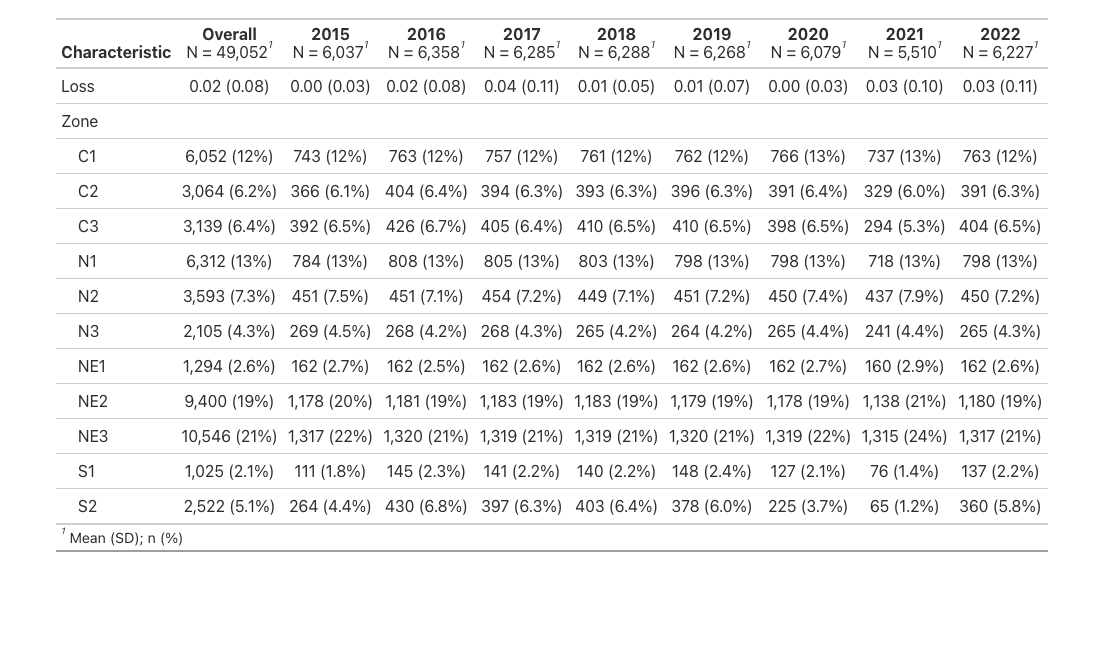
\includegraphics[width=\textwidth]{thai_summary_stats.png}
    \end{figure}
\end{frame}

\begin{frame}{Disaster Activity Map}
    \begin{figure}[h]
        \centering
        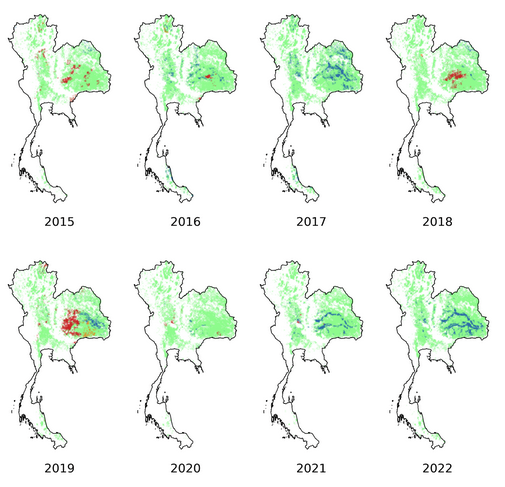
\includegraphics[width=0.6\textwidth]{disaster_map.png}
    \end{figure}
\end{frame}

\subsection{Procedure}
\begin{frame}{Evaluation Procedure}
    \begin{itemize}
        \setlength\itemsep{2em}
        \item We use leave one year out cross validation. 
        \item In each CV fold, data from year $y$ is used for testing. Data from $y'\neq y$ is used for insurance design (prediction model training and contract design).
        \item This gives us out of sample predictions for every observation in our data. We then compute utility-based performance metrics across all out of sample predictions. 
    \end{itemize}
\end{frame}

\begin{frame}{Evaluation Details}
    \begin{itemize}
        \item We use the training data and the same method to compute the premium for all methods.
        \item We modify Chen's method to use the same premium definition as ours. 
        \item We use simulated data to estimate the $\textsf{CVaR}$ when calculating the premium. 
        \item We use a CRRA utility function with $\alpha=1.5$ (\cite{flatnes2018improving}; \cite{estefania2024breaking}; \cite{jensen2019does})
    \end{itemize}
    
\end{frame}

\subsection{Framework}
\begin{frame}{Perfromance Metrics}
    \begin{itemize}
        \item We focus on the Relative Insurance Benefit (RIB) (\cite{kenduiywo2021evaluating}; \cite{estefania2024breaking}) as our main metric. 
        \item Compares a proposed insurance contract to perfect insurance. It measures the welfare gains from perfect insurance that the proposed contract recovers. 
        \item Interpretation: if RIB of an insruance $J$ is $50\%$, we can think of it as meaning that it is $50\%$ as good as perfect insurance. In other words, it yields haf as many welfare gains as perfect insurance. 
    \end{itemize}
    
\end{frame}

\begin{frame}{RIB Definition}
    Let $w^J_i$ be the wealth of farmer $i$ under insurance contract $J$. We denote perfect insurance with $PI$ and no insurance with $NI$
    \vspace{4mm}
    \begin{align*}
         CE(J):& \quad u^{-1}(\mathbb{E}[u(w^J)]) \\
         \Delta CE(J):&\quad = CE(J) - CE(NI) \\
         RIB(J):& \quad \frac{\Delta CE(J)}{\Delta CE(PI)} \\
         \text{Utility}:& \quad u(w) = \frac{1}{1-\alpha} w^{\frac{1}{1-\alpha}}
    \end{align*}
    
\end{frame}

\begin{frame}{Single Zone Evaluation Procedure}
    \begin{itemize}
        \setlength\itemsep{2em}
        \item Contract for each zone is designed as if the other zones didn't exist
        \item Required capital for zone $z$ is based only on zone $z$'s contract.  
    \end{itemize}

    \begin{align*}
        \pi_z &= \mathbb{E} \left [ \sum_z I_z \right ] + c_{\kappa} K\\
        K_z &= \sf{CVaR}_{1-\epsilon}\left ( I_z \right ) - \mathbb{E}\left [ I_z \right ]
    \end{align*}
    
\end{frame}

\subsection{Single Zone Results}
\begin{frame}{Single Zone Results}

    \begin{table}[]
        \centering
        \begin{tabular}{lllll}
        \textbf{Method} & \textbf{RIB} & \textbf{Premium} & \textbf{Cost} & \textbf{Cost PI} \\ \hline
        VMX             & 0.679        & 0.014            & 0.017         & 0.027            \\
        Chantarat       & -0.244       & 0.004            & 0.002         & 0.027            \\
        Chen            & -2.676       & 0.073            & 0.062         & 0.027           
        \end{tabular}
        \end{table}
    
\end{frame}

% \begin{frame}{Single Zone Results Key Points}
%     \begin{itemize}
%         \setlength\itemsep{2em}
%         \item Our method achieves $68\%$ of the utility gains of perfect insurance. 
%         \item Has a much lower premium and cost than Chen's method. 
%     \end{itemize}
% \end{frame}

\begin{frame}{Note on the value of $c_{\kappa}$}
    \begin{itemize}
        \setlength\itemsep{2em}
        \item Potential value for farmers is highly dependent on $c_{\kappa}$ and risk aversion, $\alpha$
        \item For the most commonly used value of $\alpha$, farmers could only benefit from perfect insurane if $c_{\kappa}=0.02$.
        \item As risk aversion increases, the gains from perfect insurance increase. 
    \end{itemize}
\end{frame}

\begin{frame}{Effects of Cost of Capital and Risk Aversion}
    \begin{figure}
        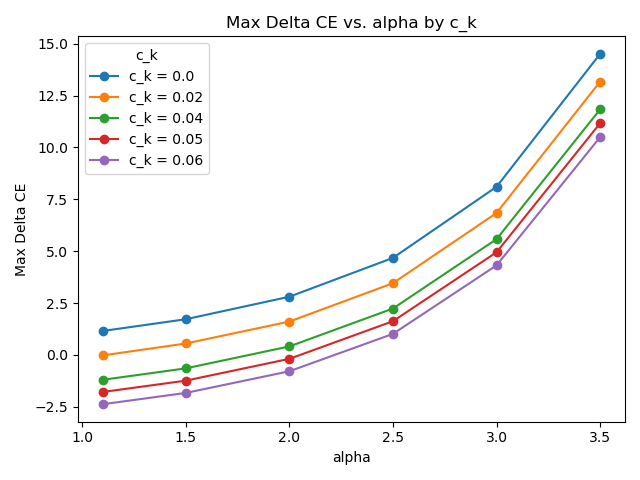
\includegraphics[width=0.75\textwidth]{../../../output/figures/Feedback/MaxDeltaCE.png}
        \caption{Perfect Insurance}
    \end{figure}
    
\end{frame}

\begin{frame}{General Insurance Behavior}
    \begin{figure}
        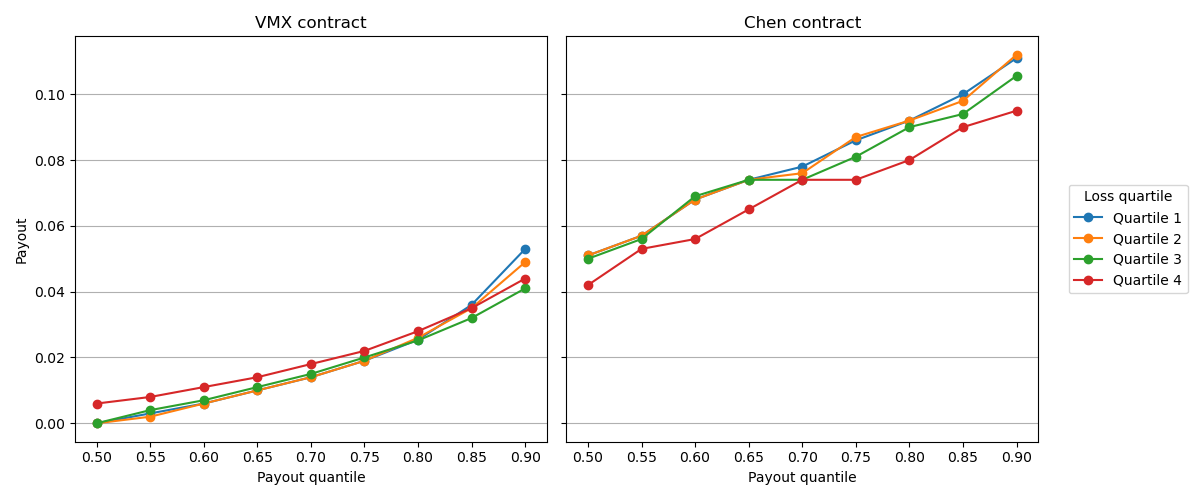
\includegraphics[width=\textwidth]{../../../output/figures/Proposal/sz_payout_by_loss_quartile.png}
        \caption{Each line shows the reverse CDF of payouts for a given loss quartile. Quartiles are numbered from smallest to largest, i.e. quartile 4 is for losses in the top quartile.}
    \end{figure}
\end{frame}

\begin{frame}{Outperforms in the in entire distribution}
    \begin{figure}
        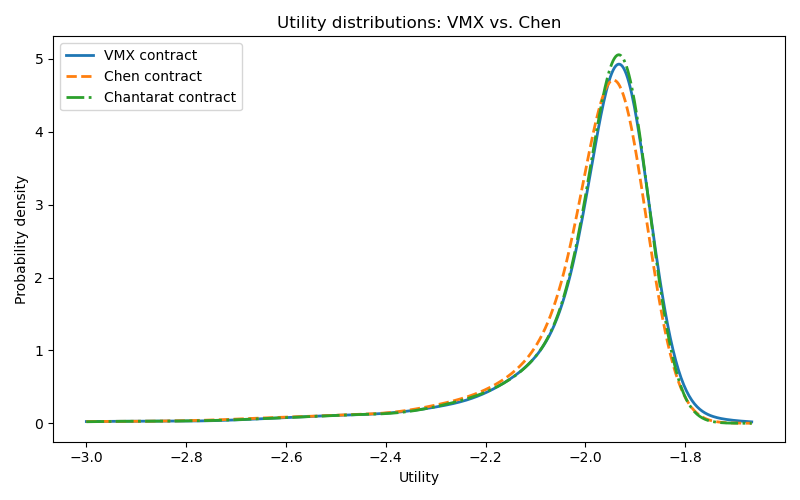
\includegraphics[width=\textwidth]{../../../output/figures/Proposal/sz_kde_plot.png}
    \end{figure}
\end{frame}

\begin{frame}{Payout and Loss Quantile Functions}
    \begin{figure}
        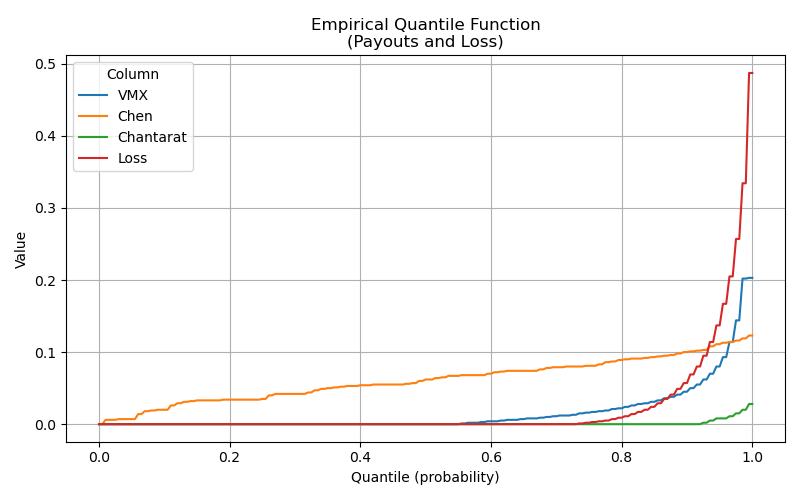
\includegraphics[width=\textwidth]{../../../output/figures/Proposal/sz_quantile_function.png}
    \end{figure}
\end{frame}

\begin{frame}{MZ vs SZ Case}
    \begin{itemize}
        \setlength \itemsep{2em}
        \item Contracts can be designed independently (Chen and Baseline) or simultaneously (VMX). 
        \item Required capital is calculated based on the portfolio of contracts
    \end{itemize}

    \begin{align*}
        \pi_z &= \mathbb{E} \left [ \sum_z I_z \right ] + c_{\kappa} \frac{\beta_z}{s_z} K\\
        K &= {\sf CVaR}_{1-\epsilon} \left ( \sum_z I_z \right ) - \mathbb{E} \left [ \sum_z I_z \right ]
    \end{align*}
    
\end{frame}

\begin{frame}{Multi zone results}
    \begin{table}[]
        \centering
        \begin{tabular}{lllll}
        \textbf{Method} & \textbf{RIB} & \textbf{Premium} & \textbf{Cost} & \textbf{Cost PI} \\ \hline
        VMX-M           & 0.592        & 0.035            & 0.036         & 0.027            \\
        VMX             & 0.524        & 0.014            & 0.017         & 0.027            \\
        Chantarat       & -0.163       & 0.004            & 0.002         & 0.027            \\
        Chen            & -1.909       & 0.074            & 0.062         & 0.027           
        \end{tabular}
        \end{table}
    
\end{frame}

\begin{frame}{SZ vz MZ Contracts}
    \begin{figure}
        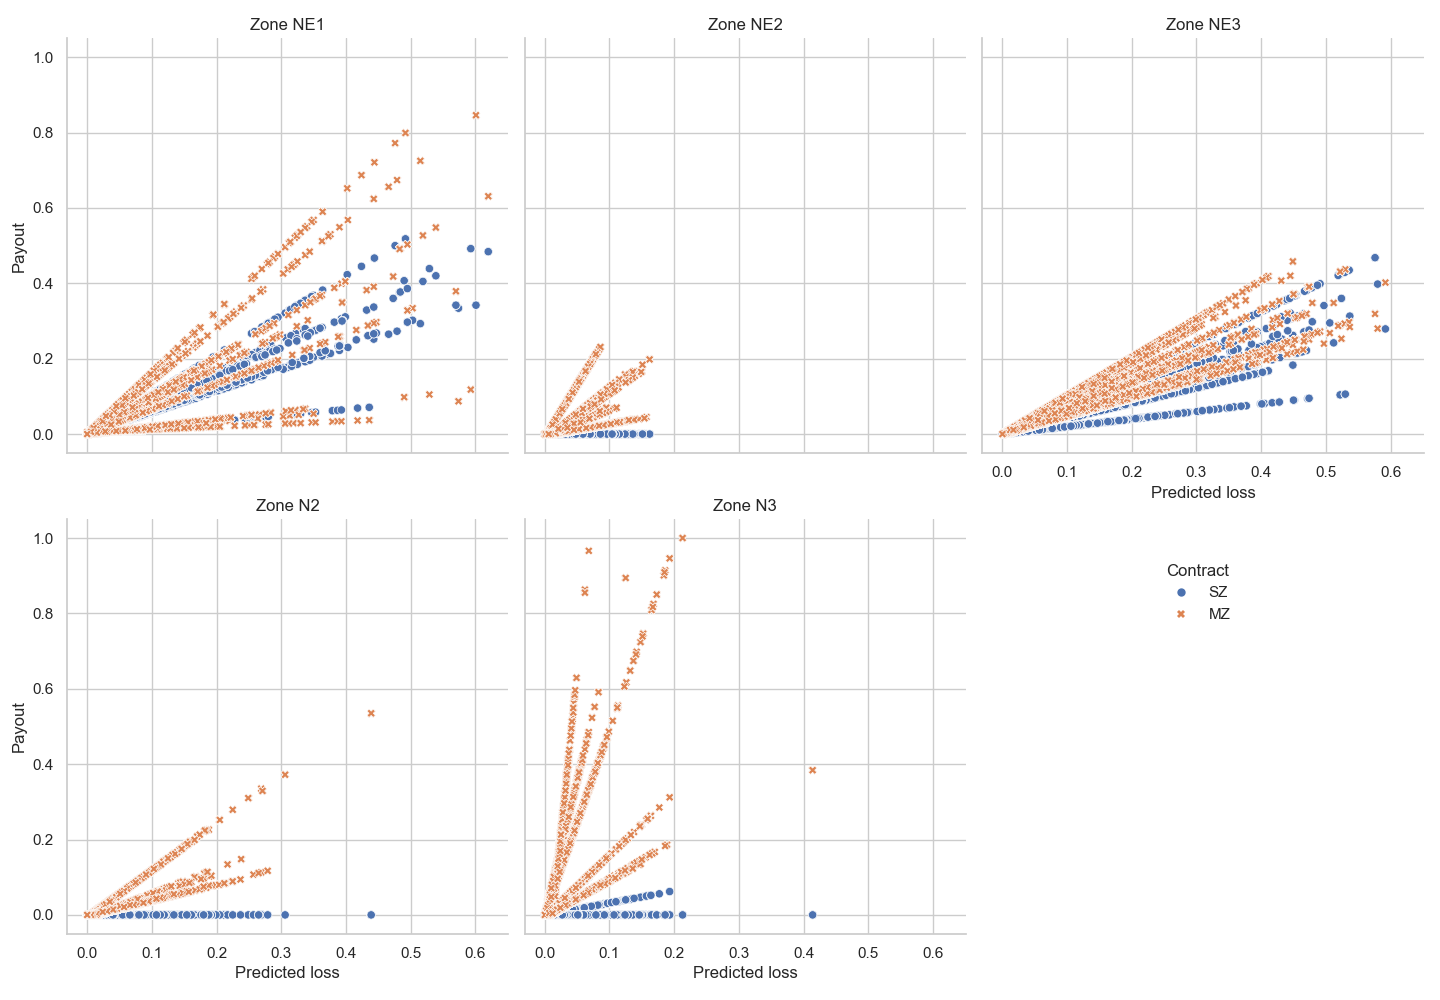
\includegraphics[width=\textwidth]{../../../output/figures/Proposal/sz_vs_mz_contracts_sns.png}
    \end{figure}
    
\end{frame}

\begin{frame}{SZ vz MZ Payouts}
    \begin{figure}
        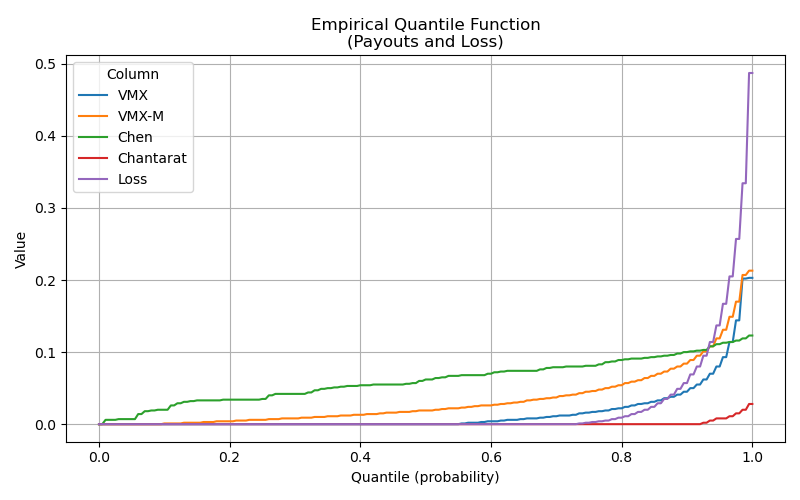
\includegraphics[width=\textwidth]{../../../output/figures/Proposal/mz_quantile_function.png}
    \end{figure}
    
\end{frame}

\begin{frame}{Capital Allocation}
    \begin{figure}
        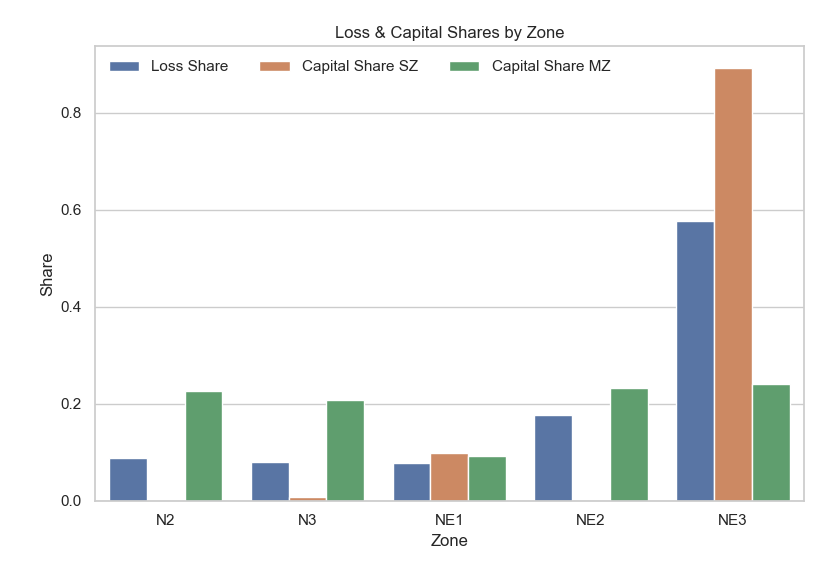
\includegraphics[width=\textwidth]{../../../output/figures/Proposal/capital_allocation.png}
    \end{figure}
    
\end{frame}


\begin{frame}{Insurance Behavior}
    Payout Precision: share of all payouts that are "valid". 

    \begin{align*}
        P = \frac{\sum_{i: \hat{y_i} > 0} w_i \hat{y_i} \min \{\ell_i, \hat{y_i}\}}{\sum_{i: \hat{y_i} > 0} w_i \hat{y_i}}
    \end{align*}

    Loss Recall: ratio of valid payouts to loss. 
    \begin{align*}
        R =  \frac{\sum_{i: \hat{y_i} > 0} w_i \hat{y_i} \min\{\ell_i, \hat{y_i}\}}{\sum_{i: \hat{y_i} > 0} w_i \ell_i}
    \end{align*}
    
\end{frame}

\begin{frame}{Good Gains and Bad Losses}
    \begin{table}[]
        \centering
        \begin{tabular}{lll}
                                     & Utility Gain           & Utility Loss           \\ \cline{2-3} 
        \multicolumn{1}{l|}{Loss}    & \multicolumn{1}{l|}{\cmark} & \multicolumn{1}{l|}{-} \\ \cline{2-3} 
        \multicolumn{1}{l|}{No Loss} & \multicolumn{1}{l|}{-} & \multicolumn{1}{l|}{\xmark} \\ \cline{2-3} 
        \end{tabular}
        \end{table}

        \cmark: utility gain during loss $\rightarrow$ "good gain"\\
        \xmark: utility loss during loss $\rightarrow$ "bad loss"
\end{frame}

% \begin{frame}{Insurance Behavior contd.}
%     \begin{itemize}
%         \item Utility gains relative to no insurance can happen when there is loss (insurance working properly) or when there is no loss (because the insurance incorrectly issued a payout).
%         \item Similarly, utility losses relative to no insurance can happen when there is no loss (due to farmers having to pay a premium) or when there is loss (because the insurance did not issue a payout).
%         \item Pct Valid Utility Gains: share of utility gains that happen when there is loss.
%         \item Pct Bad Utility Loss: share of utility losses that happen when there is loss. 
%     \end{itemize}
    
% \end{frame}

\begin{frame}{Insurance Behavior Results}
    \begin{table}[]
        \centering
        \small
        \begin{tabular}{llllll}
        Method    & RIB    & Payout Precision & Loss Recall & Good Gain & Bad Loss \\ \hline
        VMX-M     & 0.597  & 0.184            & 0.211       & 0.390          & 0.334        \\
        VMX       & 0.518  & 0.175            & 0.120       & 0.335          & 0.372        \\
        Chantarat & -0.222 & 0.328            & 0.010       & 0.616          & 0.514        \\
        Chen      & -1.924 & 0.173            & 0.298       & 0.327          & 0.440       
        \end{tabular}
        \end{table}
\end{frame}

% \begin{frame}{Caveats}
%     \begin{itemize}
%         \setlength \itemsep{2em}
%         \item Gains are concentrated in zone with larges losses
%         \item Farmers in 3/5 zones are worse off on average
%     \end{itemize}
% \end{frame}

% \begin{frame}{Caveats contd.}
    
% \end{frame}

\begin{frame}{Summary of results}
    \begin{itemize}
        \item Designing the contracts simultaneously leads to more aggressive contracts and larger utility gains.
        \item The program distributes capital costs more equitably, allowing more zones to be insured. 
        \item The resulting contracts are more efficient. 
    \end{itemize}
\end{frame}

% \section{US Midwest Evaluation}
% \begin{frame}[noframenumbering, plain]
%     \frametitle{Content}
%     \tableofcontents[currentsection]
%   \end{frame}
% \subsection{Data}
% \begin{frame}{Data}
%     Used two main data sources
%     \begin{itemize}
%         \setlength\itemsep{2em}
%         \item Illinois annual corn yield data from the National Agricultural Statistics Service (NASS). Data is available at the county level from 1925-2022. 84 counties. 
%         \item Weather data from the PRISM climate group. Has monthly data on several weather variables (temperature, precipitation, etc). Available 1895-present.
%     \end{itemize}
% \end{frame}

% \subsection{Procedure}
% \begin{frame}{Evaluation Procedure}
%     \begin{itemize}
%         \setlength\itemsep{2em}
%         \item We use a 70/15/15 train/val/test split. Data is kept in chronological order. Training data has older years and test data has the newest years. 
%         \item We modified Chen's method to use the same definition of the premium as our method. 
%         \item We use the training and validation data to design the contracts using both methods, apply the contracts to farmers in the test set, and compute performance metrics. 
%         \item We used a data shortening exercise to evaluate how the performance of both methods changed as more data became available. 
%     \end{itemize}
% \end{frame}


% \subsection{Illinois Results}
% \begin{frame}{Overview}
%     \begin{itemize}
%         \setlength\itemsep{2em}
%         \item Our method performs similarly or outperforms the Chen model when there is less than 50 years of data available.  
%         \item In terms of farmer utility, our method tends to work better with realistic data lengths. Most satellite data starts at 1980 at the earliest. 
%         \item When using data from other states, our method consistently outperforms Chen's method, but is not always better than no insurance, at least at the full premium price. This might not be a huge problem, since agricultural insurance tends to be heavily subsidized, both in rich and poor countries. In the US, it averaged $62\%$ of premiums in 2022. 
%     \end{itemize}
% \end{frame}

% % \begin{frame}{Illinois: Utility}
% %     \begin{figure}
% %         % 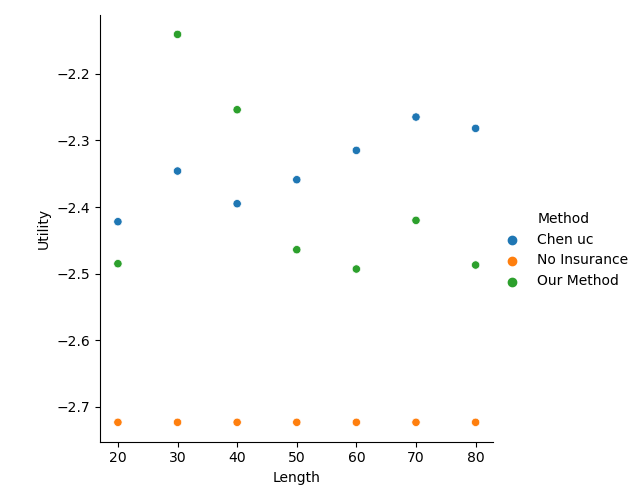
\includegraphics[width=0.75\textwidth]{../../../output/figures/Evaluation 2/Illinois_Utility_Length_ml1.png}
% %         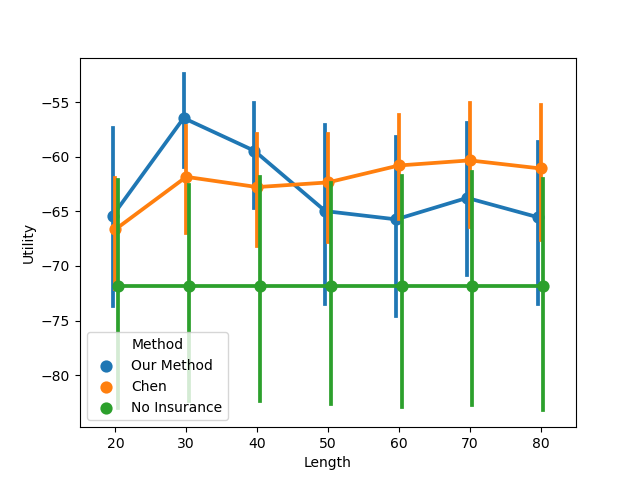
\includegraphics[width=0.75\textwidth]{../../../output/figures/Evaluation/Illinois_Average_Utility_CI.png}
% %     \end{figure}
% % \end{frame}

% \begin{frame}{Illinois Short Data (Less than 40 years)}
%     \begin{table}
%         \centering
%         \begin{tabular}{lrrr}
%             \toprule
%             Method & DeltaCE & Premium & Required Capital \\
%             \midrule
%             Chantarat & 4.13 & 113.96 & 158.73 \\
%             Chen uc & 4.87 & 60.69 & 134.35 \\
%             Our Method & 5.31 & 62.49 & 97.91 \\
%             \bottomrule
%             \end{tabular}
%     \end{table}
    
        
% \end{frame}

% \begin{frame}{Illinois Long Data (More than 40 years)}
%     \begin{table}
%         \centering
%         \begin{tabular}{lrrr}
%             \toprule
%             Method & DeltaCE & Premium & Required Capital \\
%             \midrule
%             Chantarat & 2.05 & 105.53 & 135.72 \\
%             Chen uc & 4.82 & 50.06 & 115.02 \\
%             Our Method & 3.82 & 41.75 & 67.80 \\
%             \bottomrule
%             \end{tabular}
%     \end{table}
    
% \end{frame}

% % \begin{frame}{Illinois: Insurer Cost}
% %     \begin{figure}
% %         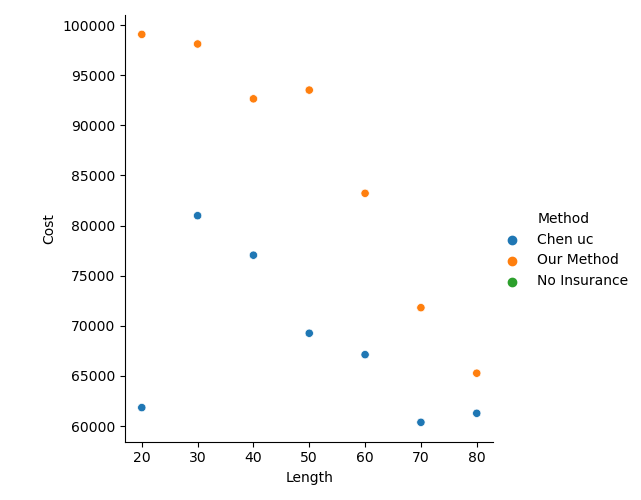
\includegraphics[width=0.75\textwidth]{../../../output/figures/Evaluation/Illinois_Cost_Length_ml1.png}

% %     \end{figure}
% % \end{frame}




% \subsection{Insuring the US Midwest}
% \begin{frame}[noframenumbering, plain]
%     \frametitle{Content}
%     \tableofcontents[currentsubsection]
%   \end{frame}


% \subsection{Multi zone Results}
% \begin{frame}{Overview}
%     \begin{itemize}
%         \item Our multiple zone model adjusts contracts based on the correlation between the insured zones. In this case, it leads to contracts that pay out more frequently, but at a lower rate. This reduces the tail risk for the insurer and reduces the amount of capital needed. 
%         \item It outperforms Chen's model and the no insurance case consistently, and has lower costs and required capital than the Chen model. 
%         \item We also wanted to compare it to using our single zone model. In the following figures, Our Method: SZ refers to using our single zone method to design the contract of each state individually, but then calculating the premium as if it was a part of the portfolio. 
%     \end{itemize}
% \end{frame}

% \begin{frame}{Midwest Short Data Results}
%     \begin{table}
%         \centering
%         \begin{tabular}{lrrr}
%             \toprule
%             Method & DeltaU & Insurer Cost & Required Capital \\
%             \midrule
%             Chantarat & 5.90 & 397,474.47 & 17720.74 \\
%             Chen uc & -8.92 & 159,928.89 & 19865.41 \\
%             Our Method & 4.18 & 150,414.21 & 9982.12 \\
%             \bottomrule
%             \end{tabular}
%     \end{table}
    
        
% \end{frame}

% \begin{frame}{Midwest Long Data Results}
%     \begin{table}
%         \centering
%         \begin{tabular}{lrrr}
%             \toprule
%             Method & DeltaU & Insurer Cost & Required Capital \\
%             \midrule
%             Chantarat & 2.40 & 389,678.99 & 16874.15 \\
%             Chen uc & 0.21 & 141651.90 & 12142.11 \\
%             Our Method & 2.50 & 99,769.84 & 5559.64 \\
%             \bottomrule
%             \end{tabular}
%     \end{table}
    
% \end{frame}

% \begin{frame}{Midwest: Overall Utility}
%     \begin{figure}
%         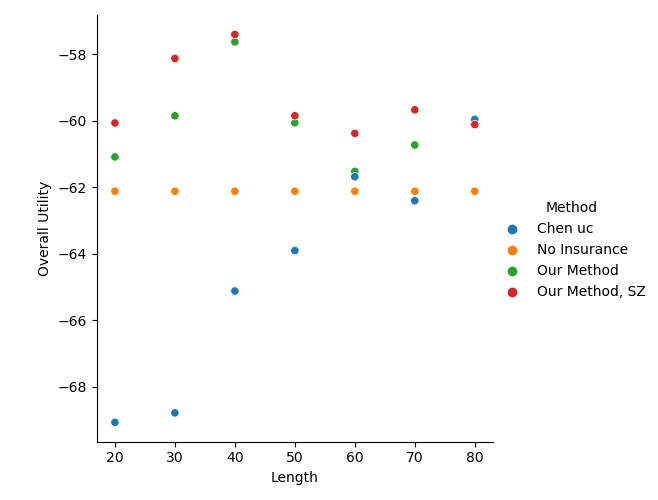
\includegraphics[width=0.75\textwidth]{../../../output/figures/Midwest Evaluation/Midwest_Overall Utility_Length.png}
%     \end{figure}
% \end{frame}

% \begin{frame}{Midwest: Insurer Cost}
%     \begin{figure}
%         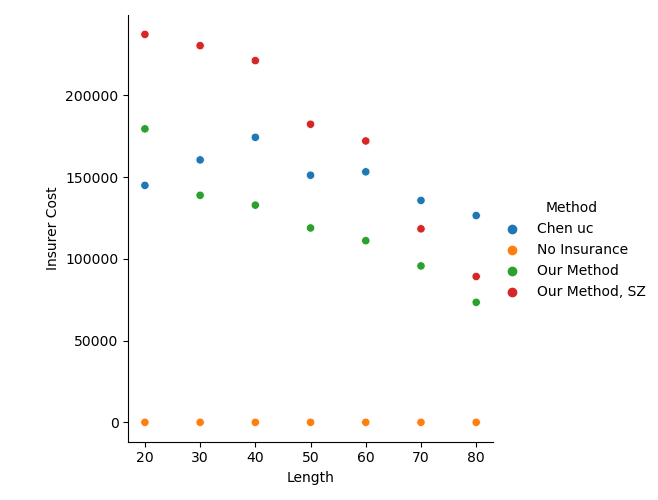
\includegraphics[width=0.75\textwidth]{../../../output/figures/Midwest Evaluation/Midwest_Insurer Cost_Length.png}
%     \end{figure}
% \end{frame}


% \section*{Moving Forward}
% \begin{frame}{Things I was thinking about adding}
%     \begin{itemize}
%         \item Deep dive as to why my method does better, and when it does better?
%         \item Run the same evaluation but with shuffled data instead of having it orderd. 
%        \item I wanted to do more of a deep dive on the benefits of taking a portfolio approach, but not sure how beyond just looking at capital requirements. Maybe using an expected return and variance approach?
%         \item A robustness check on the stability of the solutions at different dataset lengths.
%     \end{itemize}
    
% \end{frame}

% \begin{frame}{Questions}
%     \begin{itemize}
%         \item What else should I report?
%         \item How can I strengthen this evaluation?
%        \item Any robustness checks I should add?
%         \item I feel like I should do a deep dive as to why the method does
%     \end{itemize}
    
% \end{frame}

% \begin{frame}{Thai Data}
%     \begin{itemize}
%         \item Plot-level losses caused by natural disasters between 2015-2022. 
%         \item I can access the raw data, and they can send me aggregate versions as well. There are around 7000 counties in Thailand, and around 80,000 villages, the data can be aggregated at both of those levels. 
%     \end{itemize}
    
% \end{frame}

% \section*{Implementation Details}
% \begin{frame}{Loss Definition}
%     From what I can tell from the replication files, they seem to define loss in every year as: 
%     \begin{align*}
%         \ell_{st} &= R^*_s - R_{st}
%     \end{align*}

%     where $R^*_s$ is the maximum revenue observed in state $s$ across all time periods, and $R_{st}$ is the revenue in state $s$ at time $t$. 
% \end{frame}

% \begin{frame}{Initial wealth}
%     According to the paper, they set $w_0 = 389$. However, in the replication files, they set it to be $w_0 = 813 - 504 + 389$. According to the comments, $504$ is the fixed cost of operating a farm, and there are no comments regarding the $813$, I'm assuming it corresponds to $R^*$. 
% \end{frame}

% \begin{frame}{Detrending}
%     \begin{itemize}
%         \item According to the paper, they detrend the county level yield data using a 2nd order polynomial fit with a ``robust'' regression method, but they don't specify what they use, and it's not in the replication files. They also don't specify if they remove the trend using additive or multiplicative decomposition model. Using an additive decomposition model yielded the most similar losses to what they provide in the replication files. 
%         \item There are a couple of papers showing that using locally weighted regression to detrend works better. 
%     \end{itemize}
    
% \end{frame}

% \section*{Questions}
% \begin{frame}{Questions}
%     \begin{itemize}
%         \item Would it make sense to define loss as deviation from historical average? Allowing it to be positive in some years? In other words, we would first adjust all of the yield data to 2020 levels and then calculate the historical average. The loss in each year would be the deviation from this historical average. 
%         \item Should I simply follow their lead on detrending? Or should I try to improve on it?
%         \item Do you think it's necessary to show results with both definitions of the premium?
%         \item Do you think subsidy vs lump sum results would be interesting?
%     \end{itemize}
% \end{frame}

% \section*{Chen Premium Results}
% \subsection*{Illinois Results}
% \begin{frame}{Their Defn of Premium: Illinois Utility}
%     \begin{figure}
%         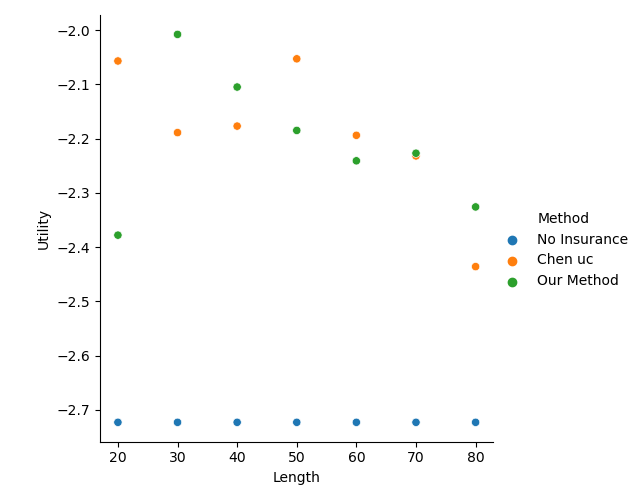
\includegraphics[width=0.75\textwidth]{../../../output/figures/Chen Premium/Illinois_Utility_Length_ml1241.png}
%     \end{figure}
% \end{frame}

% \subsection*{Iowa Results}
% \begin{frame}{Their Defn of Premium: Iowa Utility}
%     \begin{figure}
%         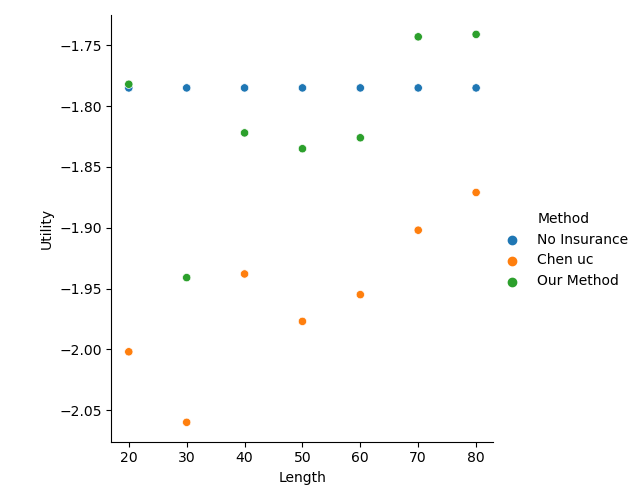
\includegraphics[width=0.75\textwidth]{../../../output/figures/Chen Premium/Iowa_Utility_Length_ml1241.png}
%     \end{figure}
% \end{frame}

% \subsection*{Missouri Results}
% \begin{frame}{Their Defn of Premium: Missouri Utility}
%     \begin{figure}
%         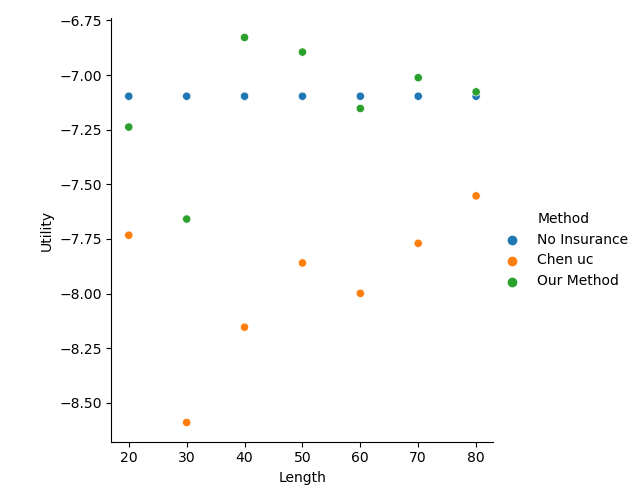
\includegraphics[width=0.75\textwidth]{../../../output/figures/Chen Premium/Missouri_Utility_Length_ml1241.png}
%     \end{figure}
% \end{frame}

% \subsection*{Indiana Results}
% \begin{frame}{Their Defn of Premium: Indiana Utility}
%     \begin{figure}
%         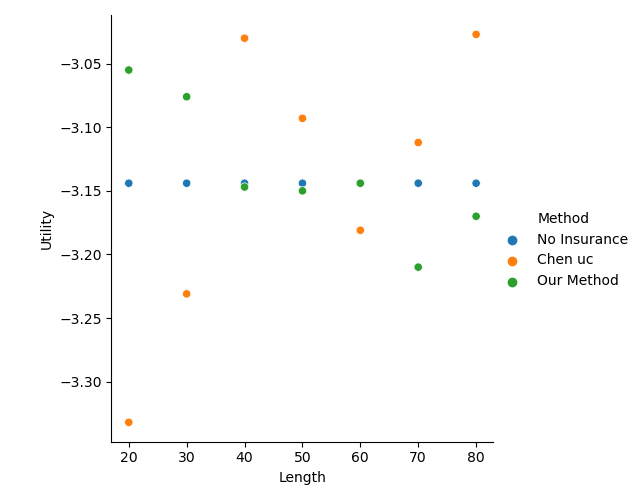
\includegraphics[width=0.75\textwidth]{../../../output/figures/Chen Premium/Indiana_Utility_Length_ml1241.png}
%     \end{figure}
% \end{frame}



% \section{Conclusion and Next Steps}
% \subsection{Conclusions}
% \begin{frame}{Conclusions}
%     \begin{itemize}
%     \setlength\itemsep{2em}
%         \item The contracts designed by our model are able to offer better protection at a similar costs, or comparable protection at lower costs than the baseline method. 
%         \item It outperforms the baseline when the prediction model is incorrectly specified and on the Kenyan pastoralist data. 
%         \item Our method is more cost effective because it takes into account spatial correlations between  areas and the costs of capital requirements. Thus, the model makes better trade offs between costs and coverage than the baseline method. 
        
%     \end{itemize}
% \end{frame}

% \subsection{Next Steps}
% \begin{frame}{Next Steps}
% \begin{itemize}
% \setlength\itemsep{2em}
%     \item We are working with practitioners to improve the model and possibly test it in practice.
%     \item We are working with the Bank of Thailand on the implementation of their satellite-based index insurance program. 
%     \item We are also talking to the International Research Institute for Climate and Society at Columbia, they have worked on the implementation of numerous index insurance programs in Africa.   
% \end{itemize}
% \end{frame}

\begin{frame}[noframenumbering, plain]{References}
\printbibliography
\end{frame}

\begin{frame}[noframenumbering, plain]{Idealized CVaR Model}
% \label{ideal-model}
\begin{itemize}
    \item \textbf{Objective:} conditional value at risk of the farmers' loss net of insurance.
    \item  \textbf{Constraint 1:} piecewise linear structure of the contract. 
    \item \textbf{Constraint 2:} budget constraint.
    \item \textbf{Constraint 3:} definition of required capital.
\end{itemize}
 
\begin{align}
        \min_{a,b,\pi, K}  & \quad CVaR_{1-\epsilon}\left ( \ell - I(\theta) \right ) \notag\\
        \text{s.t.   }I(\theta) &= \min \{ (a\hat{\ell}(\theta) + b)^+,P \} \\
        \mathbb{E}\left [ I(\theta) \right ] &+ c_{\kappa} K \leq B \\
        K &= \left( CVaR_{1-\epsilon}\left ( I(\theta) \right ) - \mathbb{E}[I(\theta)] \right) \label{cons-budget}
    \end{align}
\end{frame}

\begin{frame}[noframenumbering, plain]{The problem is non-convex, so we need convex approximations}
\label{convex-approx}
We use the following approximations of $I(\theta)$ to make the problem convex: 
\begin{align*}
    \overline{I(\theta)} &\triangleq \max \left \{ 0,a\hat{\ell}(\theta) + b\right \} \\
    \underline{I(\theta)} &\triangleq \min \{ a\hat{\ell}(\theta) + b,K \}
\end{align*}
\begin{itemize}
    \item Note that $\overline{I(\theta)} \geq I(\theta)$ and $\overline{I(\theta)}$ is convex. Conversely, $\underline{I(\theta)} \leq I(\theta)$ and $\underline{I(\theta)}$ is concave. 
    \item We replace $I(\theta)$ with either $\overline{I(\theta)}$ or $\underline{I(\theta)}$ where necessary to obtain conservative and convex approximations. 
    \item We also need approximations or proxies for $E[I(\theta)]$ in constraint . We use $\pi_{SQ} = E[I_{SQ}(\theta)]$, where $I_{SQ}$ is the contract designed using the status quo method, as a proxy for $E[I(\theta)]$ in constraint .
\end{itemize}
\end{frame}



\end{document}